\documentclass[12pt, a4paper]{article}

% ─── Packages ───────────────────────────────────────────────────────────────
\usepackage[T1]{fontenc}
\usepackage[utf8]{inputenc}
\usepackage{geometry}
\usepackage{titlesec}
\usepackage{titling}
\usepackage{xcolor}
\usepackage{enumitem}
\usepackage{parskip}
\usepackage{microtype}
\usepackage{lmodern}
\usepackage{array}
\usepackage{booktabs}
\usepackage{fancyhdr}
\usepackage{hyperref}
\usepackage{graphicx}

% ─── Page geometry ───────────────────────────────────────────────────────────
\geometry{
  top    = 2.5cm,
  bottom = 2.5cm,
  left   = 2.5cm,
  right  = 2.5cm
}

% ─── Colors ──────────────────────────────────────────────────────────────────
\definecolor{oceanblue}{RGB}{0, 80, 140}
\definecolor{seafoam}{RGB}{0, 140, 160}
\definecolor{gold}{RGB}{200, 155, 30}
\definecolor{darkgray}{RGB}{50, 50, 50}
\definecolor{lightgray}{RGB}{240, 240, 240}
\definecolor{bonuscolor}{RGB}{140, 30, 30}

% ─── Section formatting ───────────────────────────────────────────────────────
\titleformat{\section}
  {\large\bfseries\color{oceanblue}\scshape}
  {}
  {0em}
  {}
  [\vspace{-0.3em}\color{seafoam}\rule{\linewidth}{1.5pt}\vspace{0.3em}]

\titleformat{\subsection}
  {\normalsize\bfseries\color{darkgray}}
  {}
  {0em}
  {}

% ─── Header / Footer ─────────────────────────────────────────────────────────
\pagestyle{fancy}
\fancyhf{}
\fancyhead[L]{\small\color{oceanblue}\textbf{Ocean Adventure: Grand Tide}}
\fancyhead[R]{\small\color{darkgray}CMP3060 --- Graphics Programming}
\fancyfoot[C]{\small\thepage}
\renewcommand{\headrulewidth}{0.4pt}
\renewcommand{\headrule}{\hbox to\headwidth{\color{seafoam}\leaders\hrule height \headrulewidth\hfill}}

% ─── Hyperref ────────────────────────────────────────────────────────────────
\hypersetup{
  colorlinks = true,
  linkcolor  = oceanblue,
  urlcolor   = seafoam
}

% ═════════════════════════════════════════════════════════════════════════════
\begin{document}
% ═════════════════════════════════════════════════════════════════════════════

% ─── Title Page ──────────────────────────────────────────────────────────────
\begin{titlepage}
  \centering
  \vspace*{2cm}

  {\huge\bfseries\color{oceanblue} OCEAN ADVENTURE}\\[0.4em]
  {\LARGE\bfseries\color{seafoam} Grand Tide}\\[0.3em]
  {\large\color{darkgray} Game Proposal}

  \vspace{1cm}
  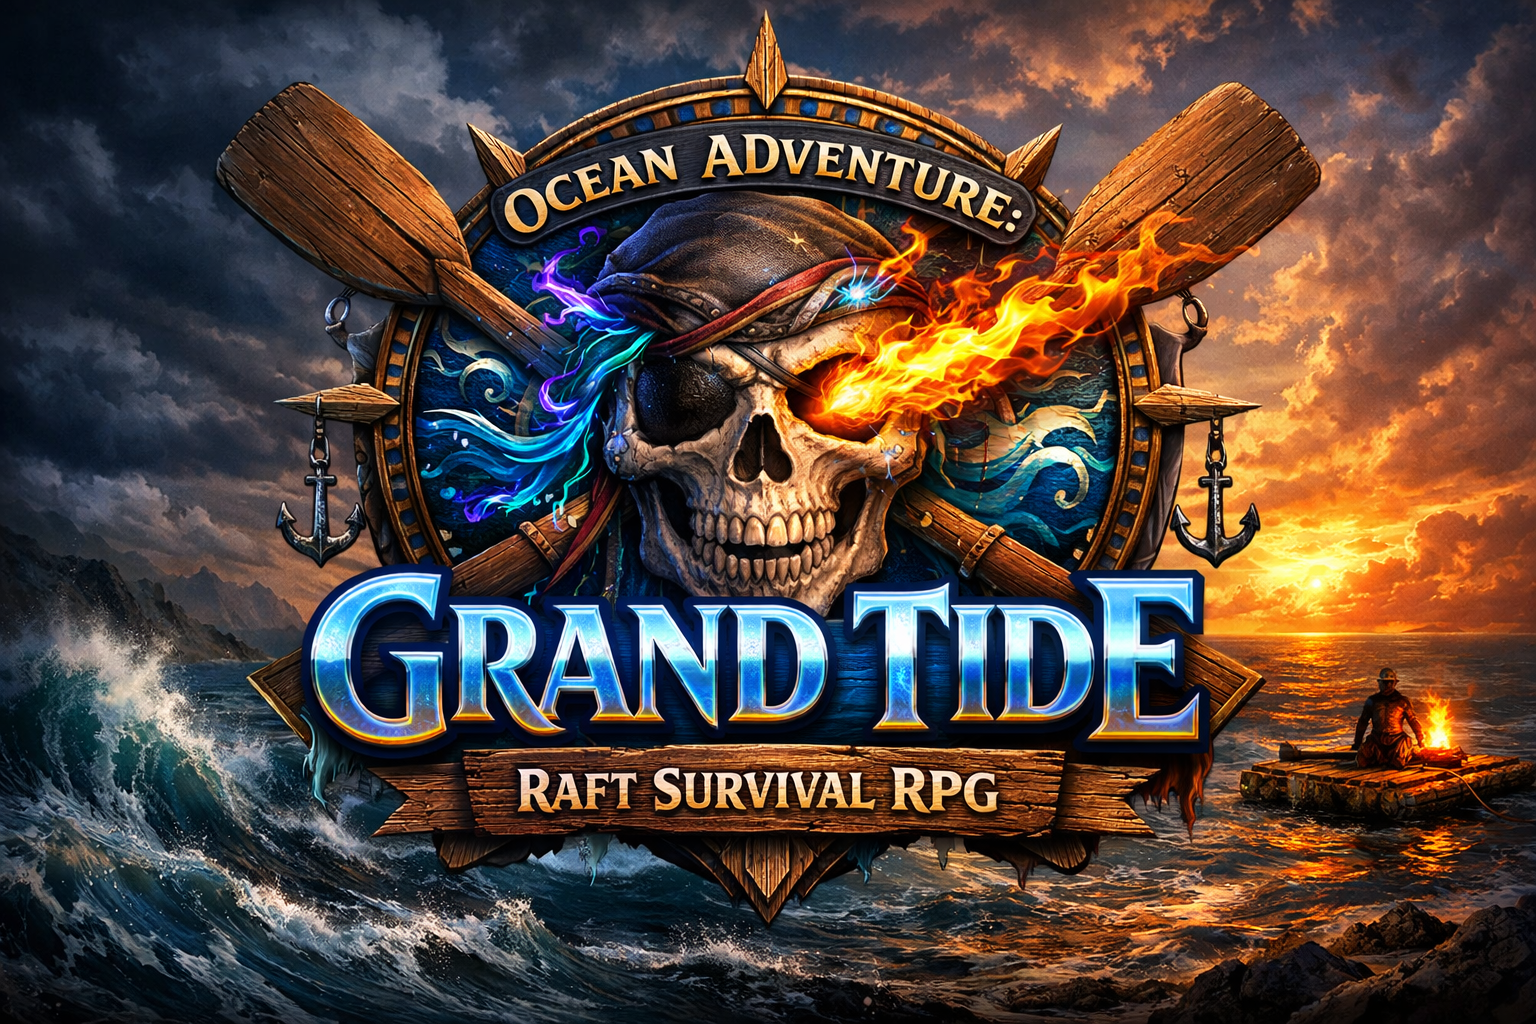
\includegraphics[width=0.65\textwidth]{grandtide.png}

  \vspace{1cm}
  {\large\color{darkgray} CMP3060: Graphics Programming}

  \vspace{1.2cm}
  \begin{tabular}{ll}
    \textbf{Mohamed Yasser} & 9230824 \\
    \textbf{Ahmed Fathy}    & 9230162 \\
    \textbf{Ahmed Gamal}    & 9230132 \\
    \textbf{Yousef Adel}    & 9231019 \\
  \end{tabular}

  \vspace{1.2cm}
  {\large Cairo University \(\cdot\) Spring 2025}

  \vfill
  {\color{seafoam}\rule{0.6\linewidth}{1.5pt}}
\end{titlepage}

% ─── Game Description ────────────────────────────────────────────────────────
\section{Game Description}

The player is stranded alone on a small wooden raft drifting across an open sea in the One Piece universe.
The goal is to survive, grow the raft, fight off threats from the ocean, and eventually reach a distant island to
find the One Piece.

The core survival loop is borrowed from the indie game \textit{Raft}: materials float past on the water surface
and must be hooked and pulled aboard, then used to expand the raft and craft tools. On top of that loop sits
the One Piece setting --- the player is a Devil Fruit user, enemies are drawn from the series, allies can be
rescued and join the crew, and the sea itself is rendered as a living, dangerous world.

% ─── Gameplay ────────────────────────────────────────────────────────────────
\section{Gameplay}

\subsection{Fishing and Hunting}
Fishing rods catch fish passively over time. The player can also actively hunt sharks that circle the raft.
Kills drop meat, fins, and occasionally rare materials.

\subsection{Devil Fruit Powers}
Devil Fruit Fragments are rare glowing items found on debris or dropped by enemies. Collecting them fills
the power gauge. The player then activates a powerful ability that clears nearby enemies. The gauge resets
after each use.

\subsection{End Goal}
After defeating the Sea King boss and a Marine fleet, the Destination Island appears. Reaching it and
completing a final encounter wins the game --- the player finds the One Piece.

% ─── Menus and UI ────────────────────────────────────────────────────────────
\section{Menus and UI}

A main menu on launch offers options to start, adjust settings, or quit. A pause menu is accessible at any time
during play with options to resume, restart, or return to the main menu.

The in-game HUD shows the player's health bar, hunger and thirst meters, the Devil Fruit power gauge, a
material counter for common resources, and a small crew panel listing rescued allies and their roles.

% ─── Technical Features ──────────────────────────────────────────────────────
\section{Technical Features}

\subsection{Water Shader}
The ocean is rendered with a custom GLSL shader. The vertex stage displaces surface positions using summed
sine waves to create rolling wave motion. The fragment stage applies a Fresnel reflection, a cubemap skybox
reflected on the water surface, refraction beneath the water plane using a framebuffer texture, and
procedural foam near the raft edges.

\subsection{3D Assets}
Every character, enemy, and prop uses an imported low-poly mesh loaded via Assimp. No primitive shapes
are used as final art.

\subsection{Entity-Component-System}
Game logic is built on a lightweight ECS framework. Spawn positions of enemies and materials, tile layout,
and crew events are randomly generated at runtime.

\subsection{Physics and Combat}
Entities move in 3D space with bounding-box collision detection. Player attacks use ray-casting to check hits
against enemy hitboxes. Sharks target the nearest foundation tile. Marine soldiers pathfind to the player once
aboard the raft.

\subsection{Lighting}
A directional light handles main world illumination using a Phong shading model. Devil Fruit Fragments carry
a local point light so they glow against the water. The sky is rendered as a cubemap skybox.

% ─── Enemies ─────────────────────────────────────────────────────────────────
\section{Enemies}

\subsection{Shark}
The most common threat. Sharks circle the raft and bite foundation tiles, dealing structural damage over time.
Killed with melee weapons or Devil Fruit. Drops meat and scales.

\subsection{Giant Octopus}
Rises from below mid-game. Tentacles slam the deck and destroy structures while the body stays submerged.
Requires ranged attacks or Devil Fruit to damage. Drops tentacle meat and devil fragments.

\subsection{Marine Ships}
Warships approach from the horizon as the raft grows. They open with cannon fire that destroys tiles in an
area. Ship size escalates from a patrol sloop early on to a full warship late in the game.

\subsection{Sea King (Boss)}
A massive sea serpent that acts as the gate to the final island. Multi-phase boss fight. Defeating it unlocks
the route to the Destination Island.

% ─── Devil Fruit System ──────────────────────────────────────────────────────
\section{Devil Fruit System}

The Devil Fruit is selected at the start of the game. Its power is unavailable until five fragments are
collected, filling the gauge. Activating it unleashes a special ability and empties the gauge.

The following fruits may be implemented (2 planned):

\begin{itemize}[leftmargin=1.5em]
  \item \textbf{Mera Mera no Mi} (Fire --- Ace) --- AOE fire burst around the player.
  \item \textbf{Gura Gura no Mi} (Quake --- Whitebeard) --- Shockwave that pushes enemies back and damages ships.
  \item \textbf{Ope Ope no Mi} (Op-Op --- Law) --- ROOM dome that slows enemies inside.
  \item \textbf{Hie Hie no Mi} (Ice --- Aokiji) --- Freezes a patch of sea, trapping nearby sharks.
  \item \textbf{Gomu Gomu no Mi} (Rubber --- Luffy) --- Reflects cannon balls and extends melee reach.
\end{itemize}

% ─── Crew System ─────────────────────────────────────────────────────────────
\section{Crew System}

Survivors in life jackets appear in the sea once the raft is large enough. The player rescues them and assigns
each one a role:

\begin{itemize}[leftmargin=1.5em]
  \item \textbf{Fisher} --- catches fish passively over time.
  \item \textbf{Guard} --- attacks nearby sharks and small enemies automatically.
  \item \textbf{Builder} --- speeds up crafting and slowly repairs damaged tiles.
  \item \textbf{Navigator} --- gives early warning when Marine ships approach.
  \item \textbf{Medic} --- slowly regenerates player health when out of combat.
\end{itemize}

Crew characters are based on the Straw Hat crew (Zoro, Nami, Usopp, Chopper, Robin).

% ─── Game Previews ───────────────────────────────────────────────────────────
\section{Game Previews}

Here are some previews from inside the game:

\begin{center}
  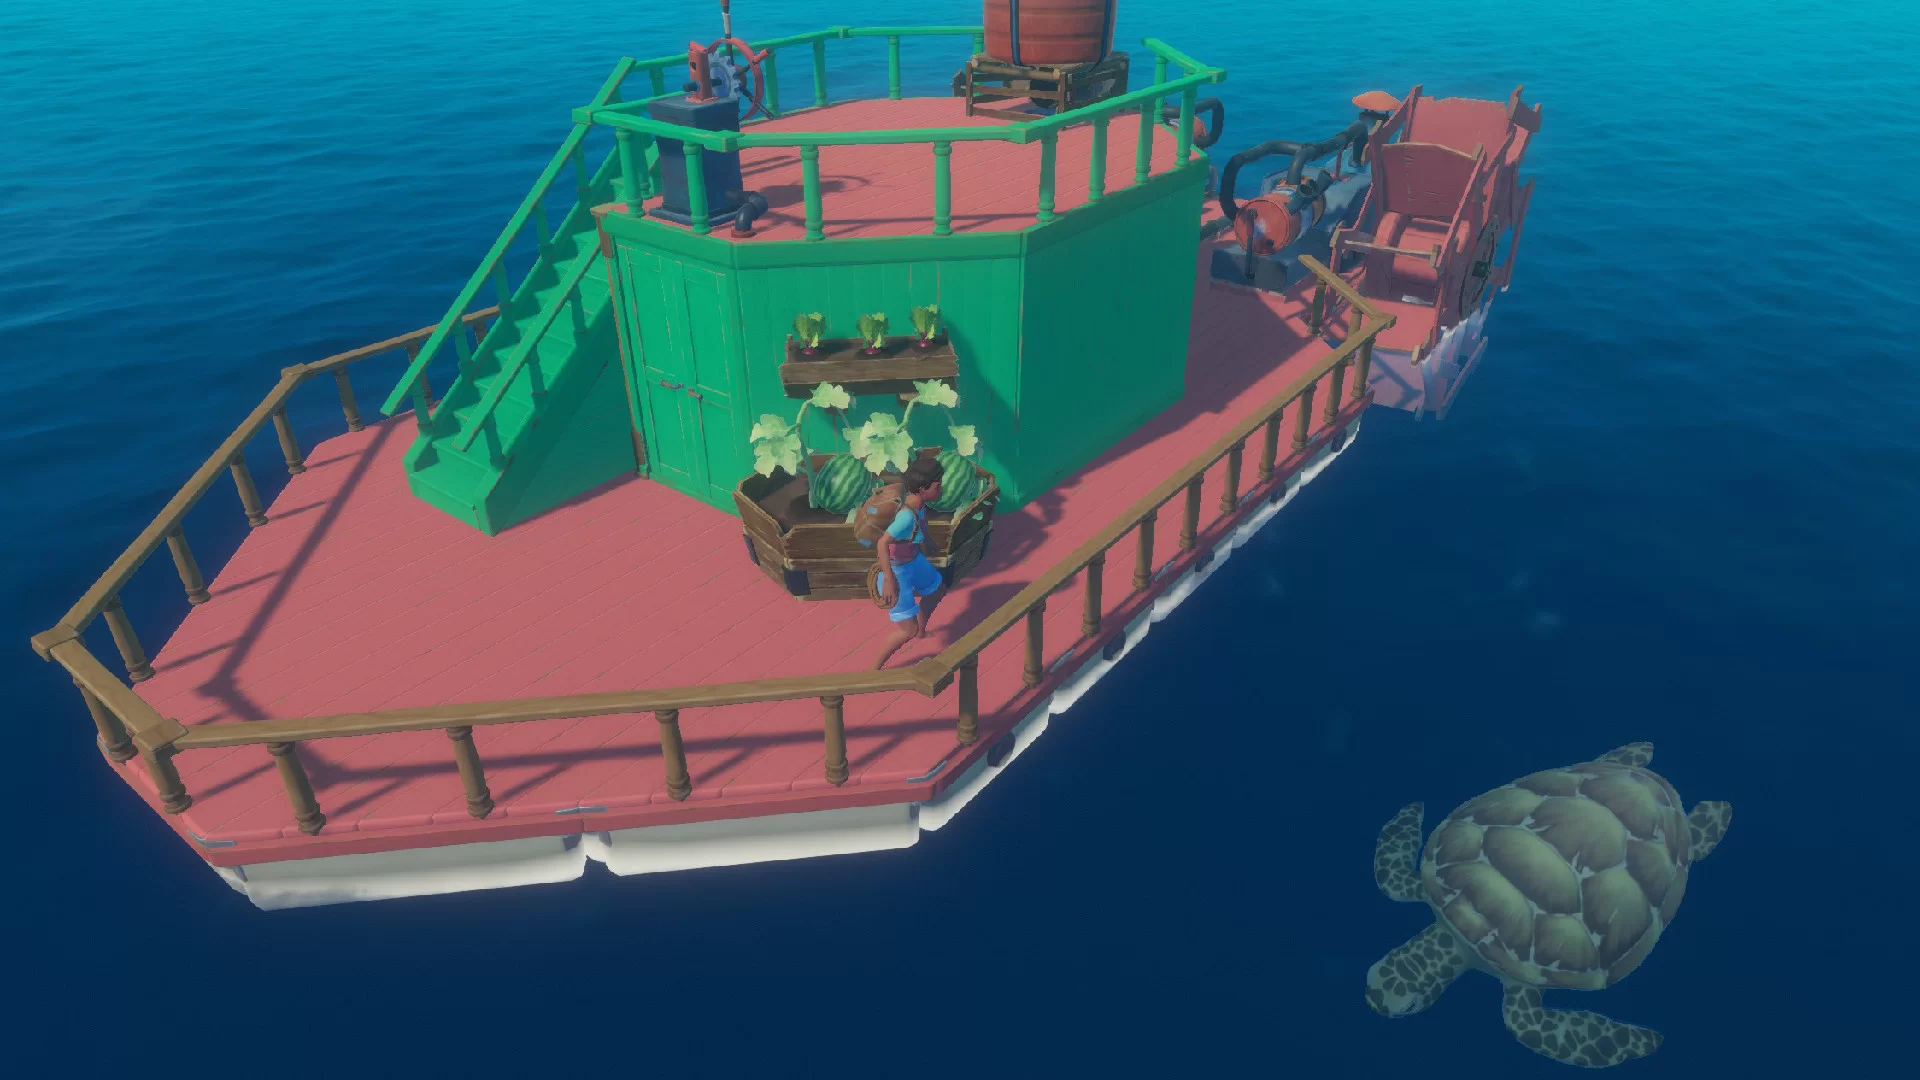
\includegraphics[width=0.7\linewidth]{I1.png}
\end{center}

\begin{center}
  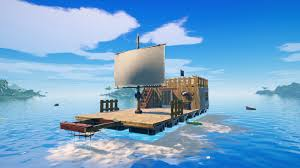
\includegraphics[width=0.7\linewidth]{I2.png}
\end{center}

\begin{center}
  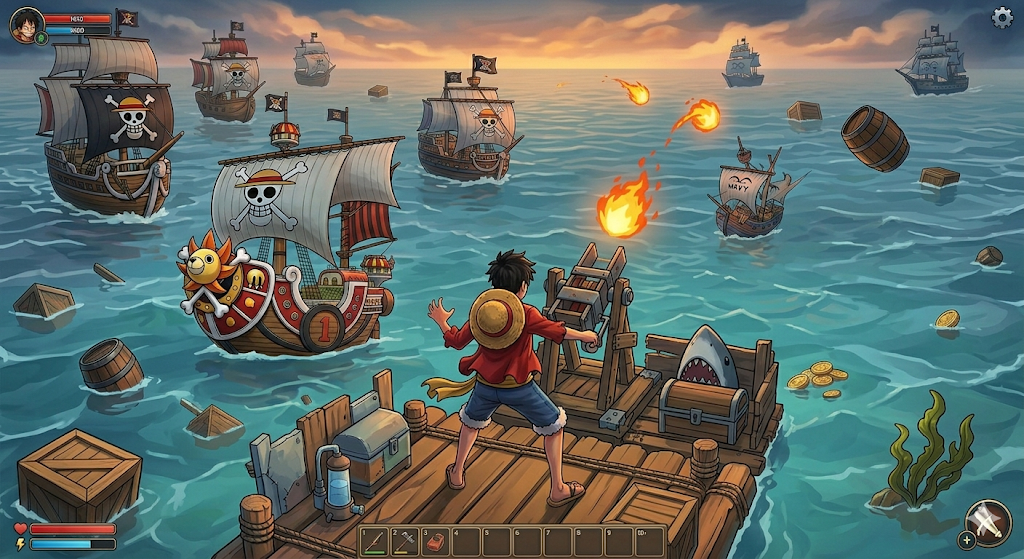
\includegraphics[width=0.7\linewidth]{I3.png}
\end{center}

% ─── Bonus Section ───────────────────────────────────────────────────────────
\newpage
\titleformat{\section}
  {\large\bfseries\color{bonuscolor}\scshape}
  {}
  {0em}
  {}
  [\vspace{-0.3em}\color{bonuscolor}\rule{\linewidth}{1.5pt}\vspace{0.3em}]

\section{Bonus Features}

The following gameplay systems are planned as bonus additions, to be implemented if time permits beyond the
core requirements.

\subsection{Collecting Materials}
Materials spawn on the sea surface and drift past the raft. The player uses a hook to grab and reel them in.
Items may include wood planks, rope, barrels, cloth, scrap metal, food, and rare Devil Fruit Fragments.

\subsection{Building and Crafting}
Materials are used to expand the raft floor one tile at a time and to craft structures: a water purifier, a
cooking grill, storage crates, and fishing rod stands.

\subsection{Rescuing Allies}
Once the raft reaches a certain size, survivors in life jackets appear in the sea. The player can rescue them
and assign them roles on the raft such as fishing, guarding, building, or navigating.

% ═════════════════════════════════════════════════════════════════════════════
\end{document}